\PassOptionsToPackage{unicode=true}{hyperref} % options for packages loaded elsewhere
\PassOptionsToPackage{hyphens}{url}
%
\documentclass[]{article}
\usepackage{lmodern}
\usepackage{amssymb,amsmath}
\usepackage{ifxetex,ifluatex}
\usepackage{fixltx2e} % provides \textsubscript
\ifnum 0\ifxetex 1\fi\ifluatex 1\fi=0 % if pdftex
  \usepackage[T1]{fontenc}
  \usepackage[utf8]{inputenc}
  \usepackage{textcomp} % provides euro and other symbols
\else % if luatex or xelatex
  \usepackage{unicode-math}
  \defaultfontfeatures{Ligatures=TeX,Scale=MatchLowercase}
\fi
% use upquote if available, for straight quotes in verbatim environments
\IfFileExists{upquote.sty}{\usepackage{upquote}}{}
% use microtype if available
\IfFileExists{microtype.sty}{%
\usepackage[]{microtype}
\UseMicrotypeSet[protrusion]{basicmath} % disable protrusion for tt fonts
}{}
\IfFileExists{parskip.sty}{%
\usepackage{parskip}
}{% else
\setlength{\parindent}{0pt}
\setlength{\parskip}{6pt plus 2pt minus 1pt}
}
\usepackage{hyperref}
\hypersetup{
            pdftitle={Stochastische Ausarbeitung},
            pdfauthor={Bela Schinke},
            pdfborder={0 0 0},
            breaklinks=true}
\urlstyle{same}  % don't use monospace font for urls
\usepackage[margin=1in]{geometry}
\usepackage{color}
\usepackage{fancyvrb}
\newcommand{\VerbBar}{|}
\newcommand{\VERB}{\Verb[commandchars=\\\{\}]}
\DefineVerbatimEnvironment{Highlighting}{Verbatim}{commandchars=\\\{\}}
% Add ',fontsize=\small' for more characters per line
\usepackage{framed}
\definecolor{shadecolor}{RGB}{248,248,248}
\newenvironment{Shaded}{\begin{snugshade}}{\end{snugshade}}
\newcommand{\AlertTok}[1]{\textcolor[rgb]{0.94,0.16,0.16}{#1}}
\newcommand{\AnnotationTok}[1]{\textcolor[rgb]{0.56,0.35,0.01}{\textbf{\textit{#1}}}}
\newcommand{\AttributeTok}[1]{\textcolor[rgb]{0.77,0.63,0.00}{#1}}
\newcommand{\BaseNTok}[1]{\textcolor[rgb]{0.00,0.00,0.81}{#1}}
\newcommand{\BuiltInTok}[1]{#1}
\newcommand{\CharTok}[1]{\textcolor[rgb]{0.31,0.60,0.02}{#1}}
\newcommand{\CommentTok}[1]{\textcolor[rgb]{0.56,0.35,0.01}{\textit{#1}}}
\newcommand{\CommentVarTok}[1]{\textcolor[rgb]{0.56,0.35,0.01}{\textbf{\textit{#1}}}}
\newcommand{\ConstantTok}[1]{\textcolor[rgb]{0.00,0.00,0.00}{#1}}
\newcommand{\ControlFlowTok}[1]{\textcolor[rgb]{0.13,0.29,0.53}{\textbf{#1}}}
\newcommand{\DataTypeTok}[1]{\textcolor[rgb]{0.13,0.29,0.53}{#1}}
\newcommand{\DecValTok}[1]{\textcolor[rgb]{0.00,0.00,0.81}{#1}}
\newcommand{\DocumentationTok}[1]{\textcolor[rgb]{0.56,0.35,0.01}{\textbf{\textit{#1}}}}
\newcommand{\ErrorTok}[1]{\textcolor[rgb]{0.64,0.00,0.00}{\textbf{#1}}}
\newcommand{\ExtensionTok}[1]{#1}
\newcommand{\FloatTok}[1]{\textcolor[rgb]{0.00,0.00,0.81}{#1}}
\newcommand{\FunctionTok}[1]{\textcolor[rgb]{0.00,0.00,0.00}{#1}}
\newcommand{\ImportTok}[1]{#1}
\newcommand{\InformationTok}[1]{\textcolor[rgb]{0.56,0.35,0.01}{\textbf{\textit{#1}}}}
\newcommand{\KeywordTok}[1]{\textcolor[rgb]{0.13,0.29,0.53}{\textbf{#1}}}
\newcommand{\NormalTok}[1]{#1}
\newcommand{\OperatorTok}[1]{\textcolor[rgb]{0.81,0.36,0.00}{\textbf{#1}}}
\newcommand{\OtherTok}[1]{\textcolor[rgb]{0.56,0.35,0.01}{#1}}
\newcommand{\PreprocessorTok}[1]{\textcolor[rgb]{0.56,0.35,0.01}{\textit{#1}}}
\newcommand{\RegionMarkerTok}[1]{#1}
\newcommand{\SpecialCharTok}[1]{\textcolor[rgb]{0.00,0.00,0.00}{#1}}
\newcommand{\SpecialStringTok}[1]{\textcolor[rgb]{0.31,0.60,0.02}{#1}}
\newcommand{\StringTok}[1]{\textcolor[rgb]{0.31,0.60,0.02}{#1}}
\newcommand{\VariableTok}[1]{\textcolor[rgb]{0.00,0.00,0.00}{#1}}
\newcommand{\VerbatimStringTok}[1]{\textcolor[rgb]{0.31,0.60,0.02}{#1}}
\newcommand{\WarningTok}[1]{\textcolor[rgb]{0.56,0.35,0.01}{\textbf{\textit{#1}}}}
\usepackage{longtable,booktabs}
% Fix footnotes in tables (requires footnote package)
\IfFileExists{footnote.sty}{\usepackage{footnote}\makesavenoteenv{longtable}}{}
\usepackage{graphicx,grffile}
\makeatletter
\def\maxwidth{\ifdim\Gin@nat@width>\linewidth\linewidth\else\Gin@nat@width\fi}
\def\maxheight{\ifdim\Gin@nat@height>\textheight\textheight\else\Gin@nat@height\fi}
\makeatother
% Scale images if necessary, so that they will not overflow the page
% margins by default, and it is still possible to overwrite the defaults
% using explicit options in \includegraphics[width, height, ...]{}
\setkeys{Gin}{width=\maxwidth,height=\maxheight,keepaspectratio}
\setlength{\emergencystretch}{3em}  % prevent overfull lines
\providecommand{\tightlist}{%
  \setlength{\itemsep}{0pt}\setlength{\parskip}{0pt}}
\setcounter{secnumdepth}{0}
% Redefines (sub)paragraphs to behave more like sections
\ifx\paragraph\undefined\else
\let\oldparagraph\paragraph
\renewcommand{\paragraph}[1]{\oldparagraph{#1}\mbox{}}
\fi
\ifx\subparagraph\undefined\else
\let\oldsubparagraph\subparagraph
\renewcommand{\subparagraph}[1]{\oldsubparagraph{#1}\mbox{}}
\fi

% set default figure placement to htbp
\makeatletter
\def\fps@figure{htbp}
\makeatother

\usepackage[]{natbib}
\bibliographystyle{plainnat}

\title{Stochastische Ausarbeitung}
\author{Bela Schinke}
\date{16.04.2023}

\begin{document}
\maketitle

{
\setcounter{tocdepth}{2}
\tableofcontents
}
\hypertarget{einleitung}{%
\section{Einleitung}\label{einleitung}}

Viel Spaß mit meiner Ausarbeitung :)\\
Quellen werden am Anfang jedes Kapitels aufgeführt.

Allgemeine Formulierungshilfe von \citep{ChatGPT}.\\
Text Completion für Freitext und (hauptsächlich) R Code von \citep{GithubCopilot}.\\
Das Skript von \citep{skript} wurde bei fast allen Aufgaben verwendet.

\hypertarget{aufagabe-1}{%
\section{Aufagabe 1}\label{aufagabe-1}}

\hypertarget{chi2-anpassungstest}{%
\subsection{\texorpdfstring{\(\chi^2\)-Anpassungstest}{\textbackslash{}chi\^{}2-Anpassungstest}}\label{chi2-anpassungstest}}

\hypertarget{theorieteil}{%
\subsubsection{Theorieteil}\label{theorieteil}}

\citep{wikipediaChi2}

In der Multinomialverteilung haben wir \(4\) Kategorien, welche jeweils Binomial verteilt sind.
Für große \(n\) ist die Binomialverteilung normalverteilt mit \(\mu = n \cdot p\) und \(\sigma = \sqrt{n \cdot p \cdot (1-p)}\).
Sei \(a_1, a_2, a_3, a_4\) die Anzahl der Beobachtungen in den Kategorien. Damit ist \(\dfrac{a_j-n \cdot p_j}{\sqrt{n \cdot p_j}}\sim N(0,1)\).\\
Das wegfallen des \((1-p)\) im Nenner kommt daher, dass es sich um eine Multinomialverteilung handelt.\\
Also ist \(\dfrac{(a_j-n \cdot p_j)^2}{n \cdot p_j}\sim (N(0,1))^2\)\\
Damit ist die Summe \(\sum_{j=1}^4 \dfrac{(a_j-n \cdot p_j)^2}{n \cdot p_j \cdot (1-p_j)}\sim \chi^2_3\).

Da die p-Werte der \(\chi^2\)-Verteilung bekannt sind, kann so ein einfacher Hypothesentest durchgeführt werden:

\hypertarget{anwendung}{%
\subsubsection{Anwendung}\label{anwendung}}

\[\begin{aligned}H_0: p_1 = \frac18, p_2 = \frac14, p_3 = \frac12, p_4 = \frac18  \\
H_1: p_1 \neq \frac18 \vee p_2 \neq \frac14 \vee p_3 \neq \frac12 \vee p_4 \neq \frac18\end{aligned}\]

Simulieren wir nun den Versuch:

\begin{Shaded}
\begin{Highlighting}[]
\KeywordTok{set.seed}\NormalTok{(}\DecValTok{123}\NormalTok{)}
\CommentTok{#Diese Funktion simuliert die Multinomialverteilung und berechnet die Chi2-Teststatistik}
\NormalTok{simulateAnpassungstest <-}\StringTok{ }\ControlFlowTok{function}\NormalTok{()\{}
\NormalTok{  n <-}\StringTok{ }\DecValTok{1000}
\NormalTok{  p <-}\StringTok{ }\KeywordTok{c}\NormalTok{(}\DecValTok{1}\OperatorTok{/}\DecValTok{8}\NormalTok{, }\DecValTok{1}\OperatorTok{/}\DecValTok{4}\NormalTok{, }\DecValTok{1}\OperatorTok{/}\DecValTok{2}\NormalTok{, }\DecValTok{1}\OperatorTok{/}\DecValTok{8}\NormalTok{)}
\NormalTok{  a <-}\StringTok{ }\KeywordTok{rmultinom}\NormalTok{(}\DecValTok{1}\NormalTok{, n, p)}
  \KeywordTok{sum}\NormalTok{((a }\OperatorTok{-}\StringTok{ }\NormalTok{n}\OperatorTok{*}\NormalTok{p)}\OperatorTok{^}\DecValTok{2}\OperatorTok{/}\NormalTok{(n}\OperatorTok{*}\NormalTok{p))}
\NormalTok{\}}
\end{Highlighting}
\end{Shaded}

\begin{Shaded}
\begin{Highlighting}[]
\NormalTok{results <-}\StringTok{ }\KeywordTok{c}\NormalTok{()}
\CommentTok{#Wir berechnen 300-mal die Teststatistik und speichern sie in results}
\ControlFlowTok{for}\NormalTok{ (i }\ControlFlowTok{in} \DecValTok{1}\OperatorTok{:}\DecValTok{300}\NormalTok{)\{}
\NormalTok{  results =}\KeywordTok{c}\NormalTok{(results ,}\KeywordTok{simulateAnpassungstest}\NormalTok{())}
\NormalTok{\}}
\end{Highlighting}
\end{Shaded}

\begin{Shaded}
\begin{Highlighting}[]
\CommentTok{#Wir plotten die Verteilung der Teststatistik }
\CommentTok{#und vergleichen sie mit der Chi2-Verteilung mit 3 Freiheitsgraden}
\KeywordTok{hist}\NormalTok{(results, }\DataTypeTok{freq=}\OtherTok{FALSE}\NormalTok{, }\DataTypeTok{main =} \StringTok{"Histogramm der Chi2 Werte"}\NormalTok{, }\DataTypeTok{xlab =} \StringTok{"Chi2-Wert"}\NormalTok{,}
     \DataTypeTok{ylab =} \StringTok{"relative Häufigkeit"}\NormalTok{, }\DataTypeTok{ylim =} \KeywordTok{c}\NormalTok{(}\DecValTok{0}\NormalTok{, }\FloatTok{0.25}\NormalTok{))}
\KeywordTok{curve}\NormalTok{(}\KeywordTok{dchisq}\NormalTok{(x, }\DecValTok{3}\NormalTok{), }\DataTypeTok{add =} \OtherTok{TRUE}\NormalTok{, }\DataTypeTok{col =} \StringTok{"red"}\NormalTok{)}
\end{Highlighting}
\end{Shaded}

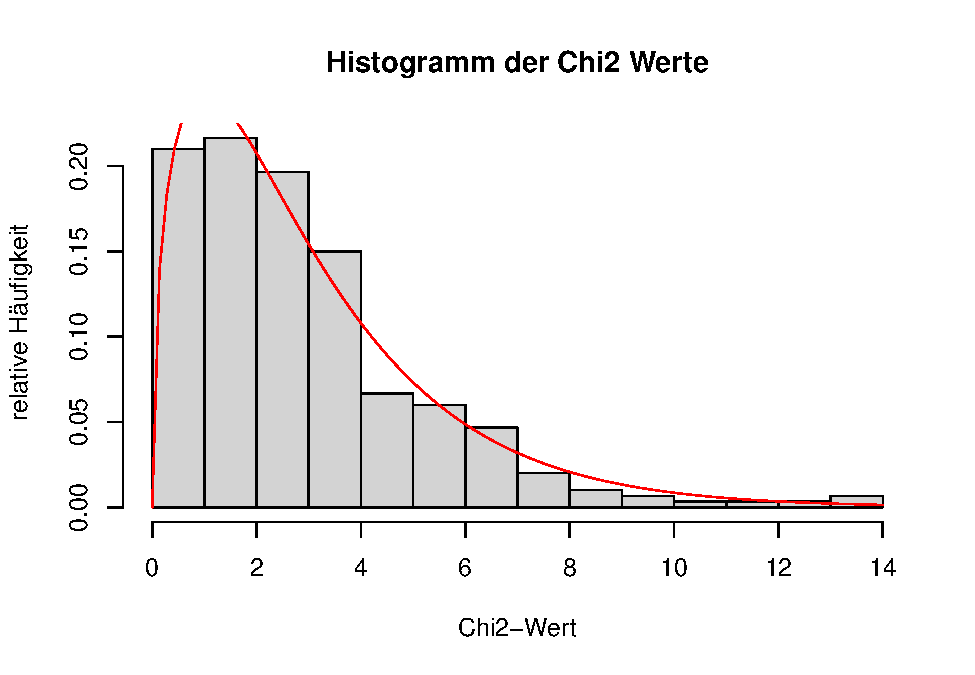
\includegraphics{Test_files/figure-latex/unnamed-chunk-3-1.pdf}

\hypertarget{t-test-mit-unbekannter-varianz}{%
\subsection{\texorpdfstring{\(t-\)Test mit unbekannter Varianz}{t-Test mit unbekannter Varianz}}\label{t-test-mit-unbekannter-varianz}}

\hypertarget{theorieteil-1}{%
\subsubsection{Theorieteil}\label{theorieteil-1}}

\citep{wikipediaT}\\
Beim zweiseitigen \(t-\)Test mit unbekannter Varianz wird die Nullhypothese \(H_0: \mu = \mu_0\) gegen die Alternative \(H_1: \mu \neq \mu_0\) getestet.
Als Teststatistik wird \(\dfrac{\sqrt{n}(\bar X_n-\mu_0)}{S_n}\) verwendet.\\
Herleitung:\\
Seien \(X_1, X_2, \dots, X_n\sim N(\mu, \sigma^2)\) unabhängig und identisch verteilt.\\
Das arithmetische Mittel \(\bar X_n\) ist normalverteilt mit \(\mu = \mu\) und \(\sigma = \dfrac{\sigma}{\sqrt{n}}\).\\
Bei bekannter Varianz wäre \(\sqrt{n}\dfrac{\bar X_n-\mu_0}{\sigma}\sim N(0,1)\).
Wir müssen allerdings die Varianz mit der empirischen Varianz ersetzen, also ist \(\sqrt{n}\dfrac{\bar X_n-\mu_0}{S_n}\sim t_{n-1}\).(T-Verteilung folgt aus Störung durch die Varianzschätzung, Skript 4.55)

Das heißt für den Test müssen wir nur die Teststatistik \(T=\dfrac{\sqrt{n}(\bar X_n-\mu_0)}{S_n}\) berechnen und anschließend deren \(p\)-Wert bestimmen. Wenn dieser kleiner als \(1-\alpha\) ist,
wird die Nullhypothese verworfen.

\hypertarget{anwendung-1}{%
\subsubsection{Anwendung}\label{anwendung-1}}

Test:

\begin{Shaded}
\begin{Highlighting}[]
\KeywordTok{set.seed}\NormalTok{(}\DecValTok{123}\NormalTok{)}
\NormalTok{mu0 <-}\StringTok{ }\DecValTok{2}
\NormalTok{sigma <-}\StringTok{ }\DecValTok{4}
\NormalTok{data <-}\StringTok{ }\KeywordTok{rnorm}\NormalTok{(}\DecValTok{1000}\NormalTok{, mu0, sigma)}
\NormalTok{alpha <-}\StringTok{ }\FloatTok{0.05}

\CommentTok{#Berechne mean und varianz der Daten}
\NormalTok{dataVar <-}\StringTok{ }\KeywordTok{var}\NormalTok{(data)}
\NormalTok{dataMean <-}\StringTok{ }\KeywordTok{mean}\NormalTok{(data)}

\CommentTok{#Berechne Teststatistik}
\NormalTok{T <-}\StringTok{ }\KeywordTok{sqrt}\NormalTok{(}\KeywordTok{length}\NormalTok{(data))}\OperatorTok{*}\NormalTok{(dataMean}\OperatorTok{-}\NormalTok{mu0)}\OperatorTok{/}\KeywordTok{sqrt}\NormalTok{(dataVar)}

\CommentTok{#Teststatistik}
\KeywordTok{print}\NormalTok{(}\KeywordTok{paste}\NormalTok{(}\StringTok{"T = "}\NormalTok{, T))}
\end{Highlighting}
\end{Shaded}

\begin{verbatim}
## [1] "T =  0.514279000759497"
\end{verbatim}

\begin{Shaded}
\begin{Highlighting}[]
\CommentTok{#p-Wert von T}
\KeywordTok{print}\NormalTok{(}\KeywordTok{paste}\NormalTok{(}\StringTok{"p-Wert von T = "}\NormalTok{, }\KeywordTok{pt}\NormalTok{(T, }\KeywordTok{length}\NormalTok{(data)}\OperatorTok{-}\DecValTok{1}\NormalTok{, }\DataTypeTok{lower.tail =} \OtherTok{FALSE}\NormalTok{)))}
\end{Highlighting}
\end{Shaded}

\begin{verbatim}
## [1] "p-Wert von T =  0.303585342303021"
\end{verbatim}

\begin{Shaded}
\begin{Highlighting}[]
\CommentTok{#Testresultat}
\ControlFlowTok{if}\NormalTok{ (}\KeywordTok{pt}\NormalTok{(T, }\KeywordTok{length}\NormalTok{(data)}\OperatorTok{-}\DecValTok{1}\NormalTok{, }\DataTypeTok{lower.tail =} \OtherTok{FALSE}\NormalTok{) }\OperatorTok{>}\StringTok{ }\DecValTok{1}\OperatorTok{-}\NormalTok{alpha)\{}
  \KeywordTok{print}\NormalTok{(}\StringTok{"Nullhypothese wird verworfen"}\NormalTok{)}
\NormalTok{\} }\ControlFlowTok{else}\NormalTok{ \{}
  \KeywordTok{print}\NormalTok{(}\StringTok{"Nullhypothese wird nicht verworfen"}\NormalTok{)}
\NormalTok{\}}
\end{Highlighting}
\end{Shaded}

\begin{verbatim}
## [1] "Nullhypothese wird nicht verworfen"
\end{verbatim}

Verteilung der Teststatistik:

\begin{Shaded}
\begin{Highlighting}[]
\KeywordTok{set.seed}\NormalTok{(}\DecValTok{123}\NormalTok{)}
\NormalTok{Tdata =}\StringTok{ }\KeywordTok{c}\NormalTok{()}

\CommentTok{#Berechne Teststatistik 300-mal}
\ControlFlowTok{for}\NormalTok{ (i }\ControlFlowTok{in} \DecValTok{1}\OperatorTok{:}\DecValTok{300}\NormalTok{)\{}
\NormalTok{  data <-}\StringTok{ }\KeywordTok{rnorm}\NormalTok{(}\DecValTok{1000}\NormalTok{, mu0, sigma)}
\NormalTok{  mu0 <-}\StringTok{ }\DecValTok{2}
\NormalTok{  alpha <-}\StringTok{ }\FloatTok{0.05}

\NormalTok{  T <-}\StringTok{ }\KeywordTok{sqrt}\NormalTok{(}\KeywordTok{length}\NormalTok{(data))}\OperatorTok{*}\NormalTok{(}\KeywordTok{mean}\NormalTok{(data)}\OperatorTok{-}\NormalTok{mu0)}\OperatorTok{/}\KeywordTok{sqrt}\NormalTok{(}\KeywordTok{var}\NormalTok{(data))}
\NormalTok{  Tdata =}\StringTok{ }\KeywordTok{c}\NormalTok{(Tdata, T)}
\NormalTok{\}}
\CommentTok{#Histogramm der Teststatistik, vergleiche mit t-Verteilung}
\KeywordTok{hist}\NormalTok{(Tdata, }\DataTypeTok{freq=}\OtherTok{FALSE}\NormalTok{, }\DataTypeTok{main =} \StringTok{"Histogramm der T Werte"}\NormalTok{,}
     \DataTypeTok{xlab =} \StringTok{"T-Wert"}\NormalTok{, }\DataTypeTok{ylab =} \StringTok{"relative Häufigkeit"}\NormalTok{)}
\KeywordTok{curve}\NormalTok{(}\KeywordTok{dt}\NormalTok{(x, }\KeywordTok{length}\NormalTok{(data)}\OperatorTok{-}\DecValTok{1}\NormalTok{), }\DataTypeTok{add =} \OtherTok{TRUE}\NormalTok{, }\DataTypeTok{col =} \StringTok{"red"}\NormalTok{)}
\end{Highlighting}
\end{Shaded}

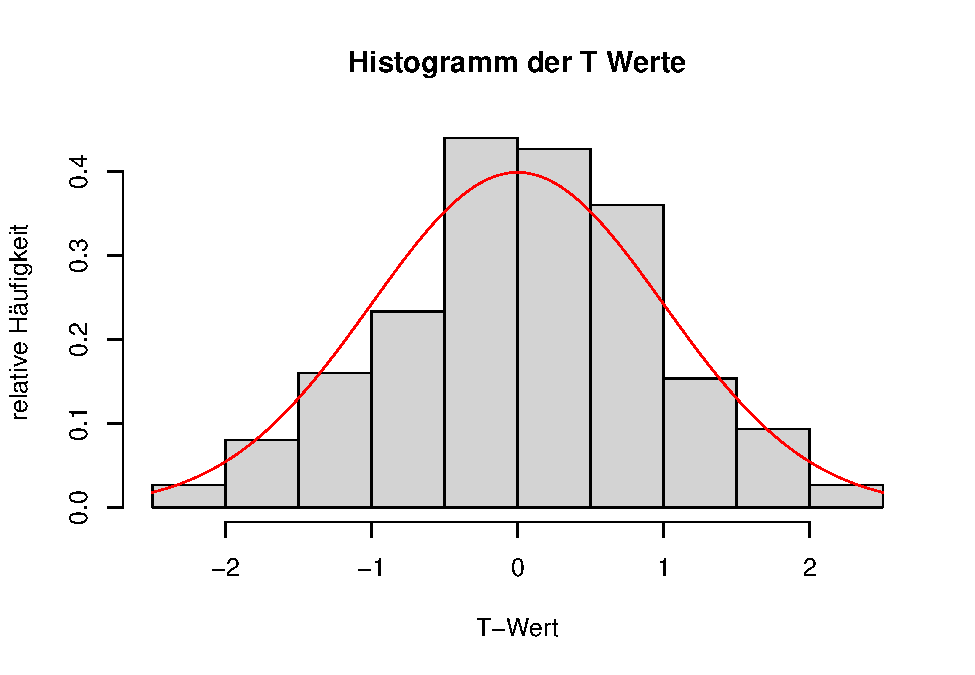
\includegraphics{Test_files/figure-latex/unnamed-chunk-5-1.pdf}

Der Kolmogorov-Smirnov-Test prüft, ob eine Stichprobe aus einer spezifischen Verteilung stammt.
Er vergleicht die empirische kumulative Verteilungsfunktion der Stichprobe mit der kumulativen
Verteilungsfunktion der Population und berechnet den maximalen Abstand zwischen den beiden Funktionen.

\begin{Shaded}
\begin{Highlighting}[]
\CommentTok{#Kolmogorov-Smirnoff-Test}
\KeywordTok{print}\NormalTok{(}\KeywordTok{ks.test}\NormalTok{(Tdata, }\StringTok{"pt"}\NormalTok{, }\KeywordTok{length}\NormalTok{(data)}\OperatorTok{-}\DecValTok{1}\NormalTok{))}
\end{Highlighting}
\end{Shaded}

\begin{verbatim}
## 
##  One-sample Kolmogorov-Smirnov test
## 
## data:  Tdata
## D = 0.068075, p-value = 0.124
## alternative hypothesis: two-sided
\end{verbatim}

Da der \(p\)-Wert des Kolmogorov-Smirnoff-Tests kleiner als \(1-\alpha=0.95\) ist, kann die Nullhypothese nicht verworfen werden,
also ist die Verteilung der Teststatistik t-verteilt.

QQ-Plot:

\begin{Shaded}
\begin{Highlighting}[]
\KeywordTok{qqnorm}\NormalTok{(Tdata)}
\KeywordTok{qqline}\NormalTok{(Tdata)}
\end{Highlighting}
\end{Shaded}

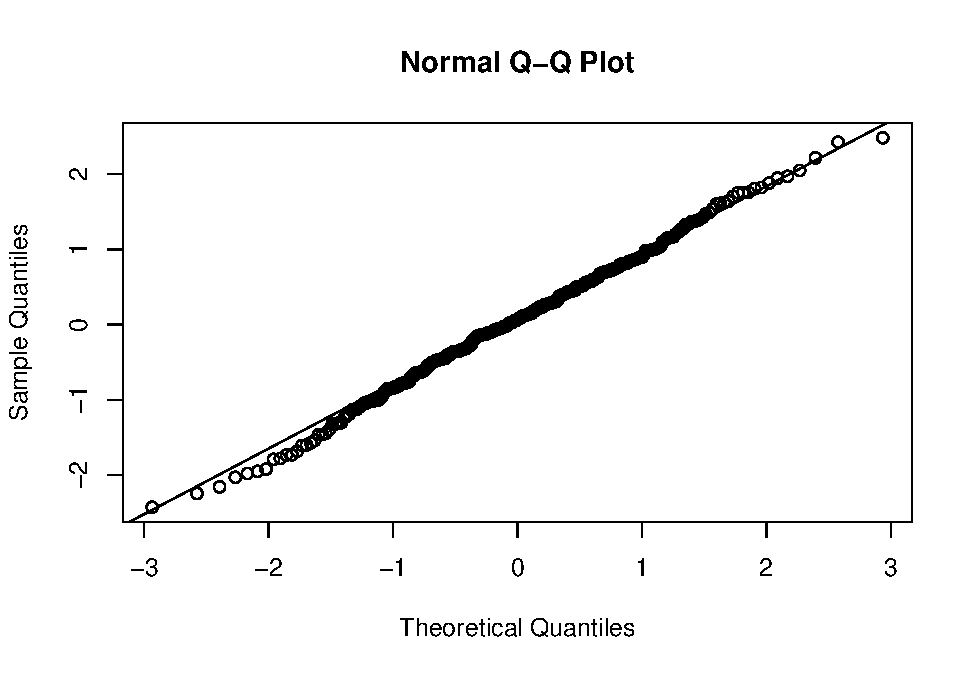
\includegraphics{Test_files/figure-latex/unnamed-chunk-7-1.pdf}
Ergebnis: Alles deutet darauf hin, dass die Teststatistik t-verteilt ist.

\hypertarget{t-test-mit-bekannter-varianz}{%
\subsection{\texorpdfstring{\(t-\)Test mit bekannter Varianz}{t-Test mit bekannter Varianz}}\label{t-test-mit-bekannter-varianz}}

\hypertarget{theorieteil-2}{%
\subsubsection{Theorieteil}\label{theorieteil-2}}

\citep{wikipediaT}
Genau wie oben, nur dass wir die Varianz nicht schätzen müssen.
Deshalb ist die Teststatistik \(\sqrt{n}\dfrac{\bar X_n-\mu_0}{\sigma}\sim N(0,1)\).
Der Rest bleibt gleich:

\hypertarget{anwendung-2}{%
\subsubsection{Anwendung}\label{anwendung-2}}

\begin{Shaded}
\begin{Highlighting}[]
\KeywordTok{set.seed}\NormalTok{(}\DecValTok{123}\NormalTok{)}
\NormalTok{mu0 <-}\StringTok{ }\DecValTok{2}
\NormalTok{sigma <-}\StringTok{ }\DecValTok{4}
\NormalTok{data <-}\StringTok{ }\KeywordTok{rnorm}\NormalTok{(}\DecValTok{1000}\NormalTok{, mu0, sigma)}
\NormalTok{alpha <-}\StringTok{ }\FloatTok{0.05}

\NormalTok{dataMean <-}\StringTok{ }\KeywordTok{mean}\NormalTok{(data)}

\NormalTok{T <-}\StringTok{ }\KeywordTok{sqrt}\NormalTok{(}\KeywordTok{length}\NormalTok{(data))}\OperatorTok{*}\NormalTok{(dataMean}\OperatorTok{-}\NormalTok{mu0)}\OperatorTok{/}\NormalTok{sigma}

\CommentTok{#Teststatistik}
\KeywordTok{print}\NormalTok{(}\KeywordTok{paste}\NormalTok{(}\StringTok{"T = "}\NormalTok{, T))}
\end{Highlighting}
\end{Shaded}

\begin{verbatim}
## [1] "T =  0.51000790152087"
\end{verbatim}

\begin{Shaded}
\begin{Highlighting}[]
\CommentTok{#p-Wert von T unter Normalverteilung}
\KeywordTok{print}\NormalTok{(}\KeywordTok{paste}\NormalTok{(}\StringTok{"p-Wert von T = "}\NormalTok{, }\KeywordTok{pnorm}\NormalTok{(T, }\DataTypeTok{lower.tail =} \OtherTok{FALSE}\NormalTok{)))}
\end{Highlighting}
\end{Shaded}

\begin{verbatim}
## [1] "p-Wert von T =  0.305022963064507"
\end{verbatim}

\begin{Shaded}
\begin{Highlighting}[]
\CommentTok{#Testresultat}
\ControlFlowTok{if}\NormalTok{ (}\KeywordTok{pnorm}\NormalTok{(T, }\DataTypeTok{lower.tail =} \OtherTok{FALSE}\NormalTok{) }\OperatorTok{>}\StringTok{ }\DecValTok{1}\OperatorTok{-}\NormalTok{alpha)\{}
  \KeywordTok{print}\NormalTok{(}\StringTok{"Nullhypothese wird verworfen"}\NormalTok{)}
\NormalTok{\} }\ControlFlowTok{else}\NormalTok{ \{}
  \KeywordTok{print}\NormalTok{(}\StringTok{"Nullhypothese wird nicht verworfen"}\NormalTok{)}
\NormalTok{\}}
\end{Highlighting}
\end{Shaded}

\begin{verbatim}
## [1] "Nullhypothese wird nicht verworfen"
\end{verbatim}

Verteilung der Teststatistik:

\begin{Shaded}
\begin{Highlighting}[]
\KeywordTok{set.seed}\NormalTok{(}\DecValTok{123}\NormalTok{)}
\NormalTok{Tdata =}\StringTok{ }\KeywordTok{c}\NormalTok{()}

\ControlFlowTok{for}\NormalTok{ (i }\ControlFlowTok{in} \DecValTok{1}\OperatorTok{:}\DecValTok{300}\NormalTok{)\{}
\NormalTok{  data <-}\StringTok{ }\KeywordTok{rnorm}\NormalTok{(}\DecValTok{1000}\NormalTok{, mu0, sigma)}
\NormalTok{  alpha <-}\StringTok{ }\FloatTok{0.05}

\NormalTok{  T <-}\StringTok{ }\KeywordTok{sqrt}\NormalTok{(}\KeywordTok{length}\NormalTok{(data))}\OperatorTok{*}\NormalTok{(}\KeywordTok{mean}\NormalTok{(data)}\OperatorTok{-}\NormalTok{mu0)}\OperatorTok{/}\NormalTok{sigma}
\NormalTok{  Tdata =}\StringTok{ }\KeywordTok{c}\NormalTok{(Tdata, T)}
\NormalTok{\}}
\KeywordTok{hist}\NormalTok{(Tdata, }\DataTypeTok{freq=}\OtherTok{FALSE}\NormalTok{, }\DataTypeTok{main =} \StringTok{"Histogramm der T Werte"}\NormalTok{, }\DataTypeTok{xlab =} \StringTok{"T-Wert"}\NormalTok{, }\DataTypeTok{ylab =} \StringTok{"relative Häufigkeit"}\NormalTok{)}
\KeywordTok{curve}\NormalTok{(}\KeywordTok{dnorm}\NormalTok{(x), }\DataTypeTok{add =} \OtherTok{TRUE}\NormalTok{, }\DataTypeTok{col =} \StringTok{"red"}\NormalTok{)}
\end{Highlighting}
\end{Shaded}

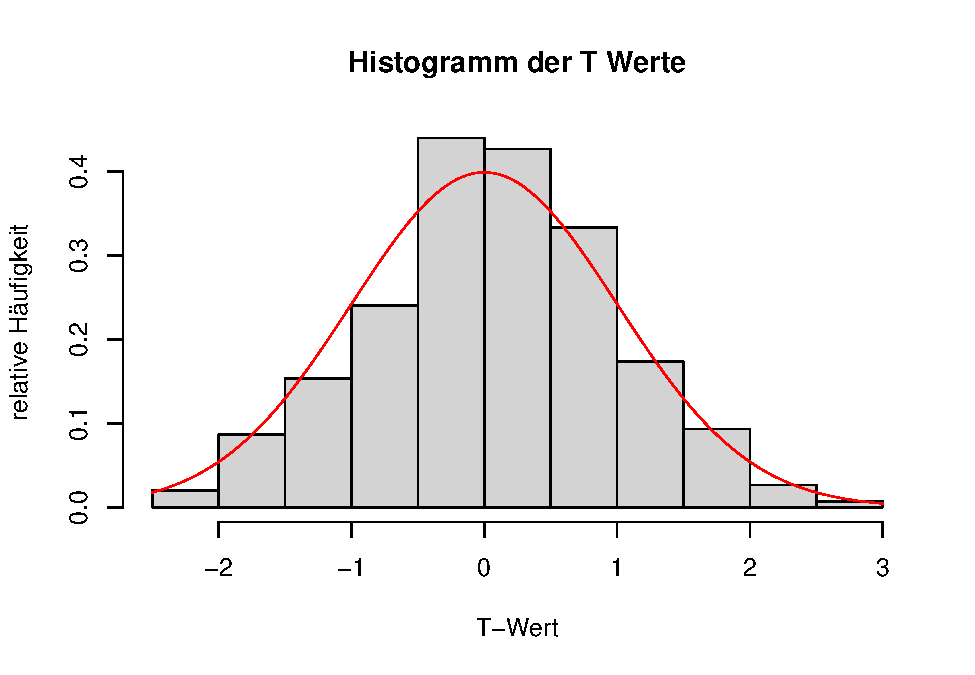
\includegraphics{Test_files/figure-latex/unnamed-chunk-9-1.pdf}

\begin{Shaded}
\begin{Highlighting}[]
\CommentTok{#Kolmogorov-Smirnoff-Test}
\KeywordTok{print}\NormalTok{(}\KeywordTok{ks.test}\NormalTok{(Tdata, }\StringTok{"pnorm"}\NormalTok{, }\DataTypeTok{lower.tail =} \OtherTok{FALSE}\NormalTok{))}
\end{Highlighting}
\end{Shaded}

\begin{verbatim}
## 
##  One-sample Kolmogorov-Smirnov test
## 
## data:  Tdata
## D = 0.99456, p-value < 2.2e-16
## alternative hypothesis: two-sided
\end{verbatim}

Da der \(p\)-Wert des Kolmogorov-Smirnoff-Tests kleiner als \(1-\alpha=0.95\) ist, kann die Nullhypothese nicht verworfen werden,
also ist die Verteilung der Teststatistik t-verteilt.

QQ-Plot:

\begin{Shaded}
\begin{Highlighting}[]
\KeywordTok{qqnorm}\NormalTok{(Tdata)}
\KeywordTok{qqline}\NormalTok{(Tdata)}
\end{Highlighting}
\end{Shaded}

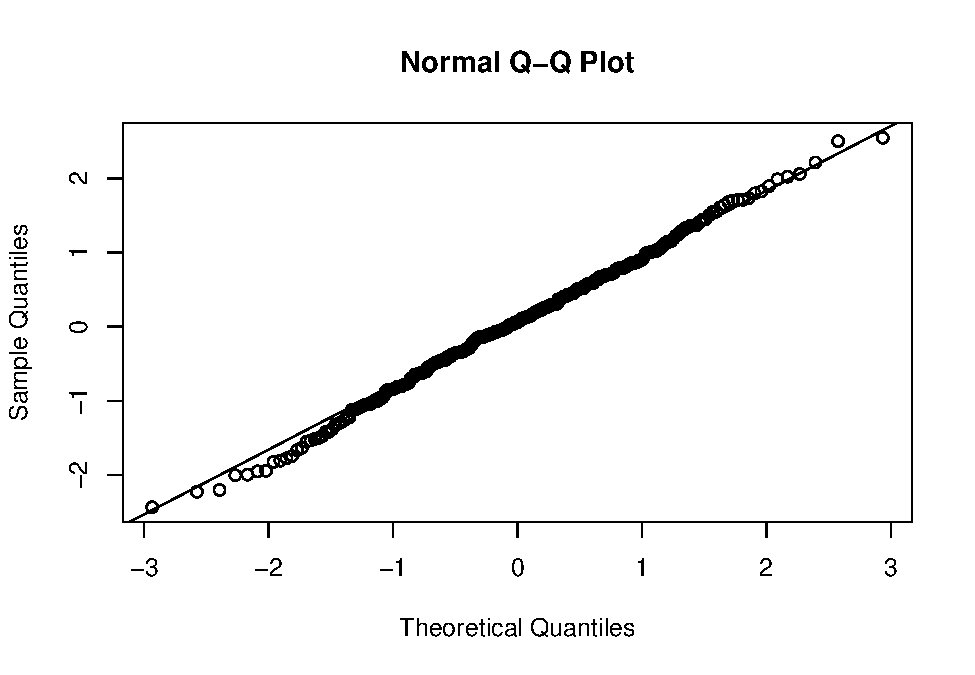
\includegraphics{Test_files/figure-latex/unnamed-chunk-10-1.pdf}
Ergebnis: Alles deutet darauf hin, dass die Teststatistik normalverteilt ist.

\hypertarget{aufgabe-2}{%
\section{Aufgabe 2}\label{aufgabe-2}}

Lineare Regression mit R

\hypertarget{theorieteil-3}{%
\subsubsection{Theorieteil}\label{theorieteil-3}}

Ein lineares Modell geht davon aus, dass eine Abhängige Variable (hier der Preis) von einer oder mehreren
unabhängigen Variablen (hier die Temperatur, der Niederschlag bei der Ernte und der Niederschlag im Winter) +
einem zufälligen Fehler erzeugt wird. Die lm-Funktion findet die Parameter, die das Modell
(nach der squared error Methode) am besten beschreiben.\\
Die Formel für das lineare Modell lautet:
\[
Y = \beta_0 + \beta_1 X_1 + \beta_2 X_2 + \beta_3 X_3 + \epsilon
\]
Die Parameter \(\beta_0, \beta_1, \beta_2, \beta_3\) werden durch die lm-Funktion bestimmt.
Die Fehlerterm \(\epsilon\) ist normalverteilt mit Erwartungswert 0 und Varianz \(\sigma^2\).

\hypertarget{anwendung-3}{%
\subsubsection{Anwendung}\label{anwendung-3}}

\hypertarget{daten-einlesen}{%
\subsection{Daten einlesen}\label{daten-einlesen}}

\begin{Shaded}
\begin{Highlighting}[]
\NormalTok{data <-}\StringTok{ }\KeywordTok{read.table}\NormalTok{(}\StringTok{"Datensaetze/wine.txt"}\NormalTok{, }\DataTypeTok{header =} \OtherTok{TRUE}\NormalTok{)}
\end{Highlighting}
\end{Shaded}

\hypertarget{uxfcberblick-uxfcber-die-daten}{%
\subsection{Überblick über die Daten}\label{uxfcberblick-uxfcber-die-daten}}

\begin{Shaded}
\begin{Highlighting}[]
\KeywordTok{head}\NormalTok{(data)}
\end{Highlighting}
\end{Shaded}

\begin{verbatim}
##   year price temp h.rain w.rain
## 1 1952    37 17.1    160    600
## 2 1953    63 16.7     80    690
## 3 1955    45 17.1    130    502
## 4 1957    22 16.1    110    420
## 5 1958    18 16.4    187    582
## 6 1959    66 17.5    187    485
\end{verbatim}

\begin{Shaded}
\begin{Highlighting}[]
\KeywordTok{summary}\NormalTok{(data)}
\end{Highlighting}
\end{Shaded}

\begin{verbatim}
##       year          price             temp           h.rain     
##  Min.   :1952   Min.   : 10.00   Min.   :15.00   Min.   : 38.0  
##  1st Qu.:1960   1st Qu.: 14.00   1st Qu.:16.15   1st Qu.: 88.0  
##  Median :1967   Median : 22.00   Median :16.40   Median :123.0  
##  Mean   :1967   Mean   : 28.81   Mean   :16.47   Mean   :144.8  
##  3rd Qu.:1974   3rd Qu.: 35.00   3rd Qu.:17.00   3rd Qu.:185.5  
##  Max.   :1980   Max.   :100.00   Max.   :17.60   Max.   :292.0  
##      w.rain     
##  Min.   :376.0  
##  1st Qu.:543.5  
##  Median :600.0  
##  Mean   :608.4  
##  3rd Qu.:705.5  
##  Max.   :830.0
\end{verbatim}

\hypertarget{lineares-modell-erstellen}{%
\subsection{Lineares Modell erstellen}\label{lineares-modell-erstellen}}

\begin{Shaded}
\begin{Highlighting}[]
\NormalTok{model <-}\StringTok{ }\KeywordTok{lm}\NormalTok{(price }\OperatorTok{~}\StringTok{ }\NormalTok{temp }\OperatorTok{+}\StringTok{ }\NormalTok{h.rain }\OperatorTok{+}\StringTok{ }\NormalTok{w.rain, }\DataTypeTok{data =}\NormalTok{ data)}
\KeywordTok{summary}\NormalTok{(model)}
\end{Highlighting}
\end{Shaded}

\begin{verbatim}
## 
## Call:
## lm(formula = price ~ temp + h.rain + w.rain, data = data)
## 
## Residuals:
##     Min      1Q  Median      3Q     Max 
## -16.580  -8.601  -4.057   6.813  29.064 
## 
## Coefficients:
##               Estimate Std. Error t value Pr(>|t|)    
## (Intercept) -365.45179   77.63849  -4.707 9.66e-05 ***
## temp          22.50086    4.28502   5.251 2.51e-05 ***
## h.rain        -0.09296    0.03746  -2.481   0.0208 *  
## w.rain         0.06103    0.02247   2.717   0.0123 *  
## ---
## Signif. codes:  0 '***' 0.001 '**' 0.01 '*' 0.05 '.' 0.1 ' ' 1
## 
## Residual standard error: 13.33 on 23 degrees of freedom
## Multiple R-squared:  0.6421, Adjusted R-squared:  0.5954 
## F-statistic: 13.75 on 3 and 23 DF,  p-value: 2.389e-05
\end{verbatim}

In dem linearen Modell hat der Temperaturkoeffzient ein positives Vorzeichen, was bedeutet,
dass der Preis mit steigender Temperatur steigt.\\
Der Koeffizient für Niederschlag bei der Ernte hat ein negatives Vorzeichen, was bedeutet,
dass der Preis mit steigendem Niederschlag bei der Ernte sinkt.\\
Der Koeffizient für Niederschlag im Winter hat ein positives Vorzeichen, was bedeutet,
dass der Preis mit steigendem Niederschlag im Winter steigt.

\hypertarget{angepasste-werte-berechnen}{%
\subsection{Angepasste Werte berechnen}\label{angepasste-werte-berechnen}}

Die angepassten Werte sind die Werte, die das lineare Modell für die Abhängige Variable berechnet.
Sie können wir mit Hilfe der Hut-Matrix berechnen (siehe Skript 9.11):

\begin{Shaded}
\begin{Highlighting}[]
\NormalTok{X =}\StringTok{ }\KeywordTok{matrix}\NormalTok{(}\KeywordTok{c}\NormalTok{(}\KeywordTok{rep}\NormalTok{(}\DecValTok{1}\NormalTok{,}\KeywordTok{length}\NormalTok{(data}\OperatorTok{$}\NormalTok{temp)),data}\OperatorTok{$}\NormalTok{temp,data}\OperatorTok{$}\NormalTok{h.rain,data}\OperatorTok{$}\NormalTok{w.rain),}\DataTypeTok{ncol=}\DecValTok{4}\NormalTok{)}
\NormalTok{HutMatrix =}\StringTok{ }\NormalTok{X}\OperatorTok\KeywordTok{solve}\NormalTok{(}\KeywordTok{t}\NormalTok{(X)}\OperatorTok\NormalTok{X)}\OperatorTok\KeywordTok{t}\NormalTok{(X)}
\NormalTok{fittedValuesByHand =}\StringTok{ }\NormalTok{HutMatrix}\OperatorTok\NormalTok{data}\OperatorTok{$}\NormalTok{price}
\end{Highlighting}
\end{Shaded}

Vergleichen mit den aus dem linearen Modell berechneten Werten:

\begin{Shaded}
\begin{Highlighting}[]
\KeywordTok{plot}\NormalTok{(fittedValuesByHand, model}\OperatorTok{$}\NormalTok{fitted.values)}
\end{Highlighting}
\end{Shaded}

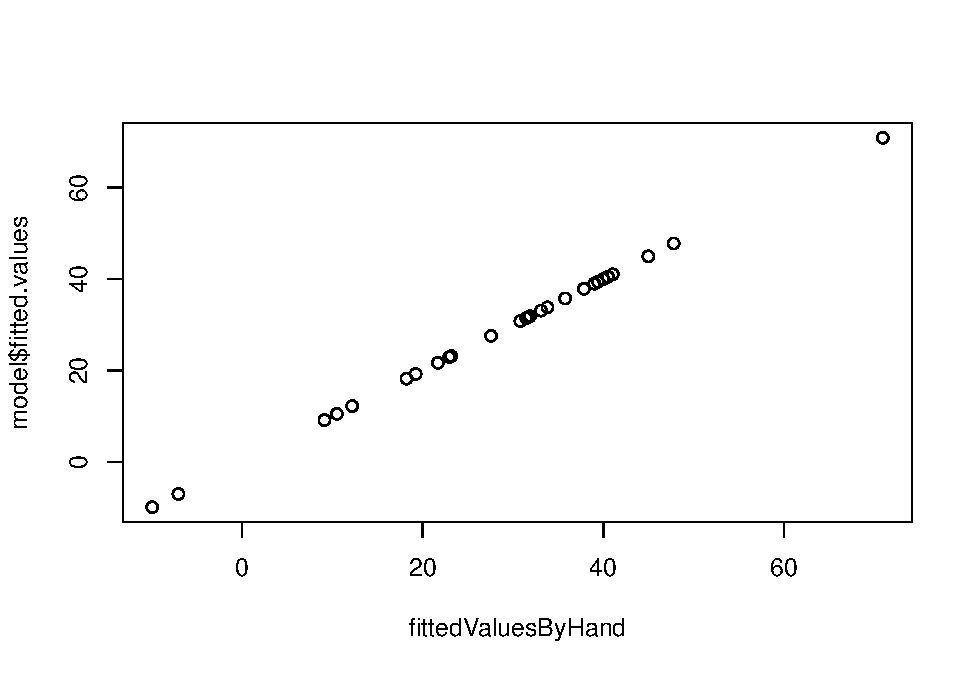
\includegraphics{Test_files/figure-latex/unnamed-chunk-15-1.pdf}

\begin{Shaded}
\begin{Highlighting}[]
\ControlFlowTok{if}\NormalTok{ (}\KeywordTok{all}\NormalTok{((fittedValuesByHand }\OperatorTok{-}\StringTok{ }\NormalTok{model}\OperatorTok{$}\NormalTok{fitted.values)}\OperatorTok{<}\FloatTok{0.0001}\NormalTok{))\{}
  \KeywordTok{print}\NormalTok{(}\StringTok{"Die beiden Werte sind annähernd gleich"}\NormalTok{)}
\NormalTok{\} }\ControlFlowTok{else}\NormalTok{ \{}
  \KeywordTok{print}\NormalTok{(}\StringTok{"Die beiden Werte sind nicht annähernd gleich"}\NormalTok{)}
\NormalTok{\}}
\end{Highlighting}
\end{Shaded}

\begin{verbatim}
## [1] "Die beiden Werte sind annähernd gleich"
\end{verbatim}

Die beiden Werte sind annähernd gleich (Unterschiede durch Rundungsfehler), was bedeutet, dass die Berechnung der angepassten Werte mit Hilfe der Hut-Matrix korrekt ist.

\hypertarget{bestimmtheitsmauxdf}{%
\subsection{Bestimmtheitsmaß}\label{bestimmtheitsmauxdf}}

Das Bestimmtheitsmaß ist ein Maß für die Güte des linearen Modells und liegt zwischen 0 und 1.
Es gibt den Anteil der Varianz durch die Regressionsvariablen an der Gesamtvarianz wieder. Grundsätzlich gilt je größer der Wert,
desto besser ist das Modell.\\
Berechne das Bestimmtheitsmaß \(R^2\) (Skript 9.16):

\begin{Shaded}
\begin{Highlighting}[]
\NormalTok{R2 =}\StringTok{ }\DecValTok{1} \OperatorTok{-}\StringTok{ }\KeywordTok{sum}\NormalTok{((data}\OperatorTok{$}\NormalTok{price }\OperatorTok{-}\StringTok{ }\NormalTok{fittedValuesByHand)}\OperatorTok{^}\DecValTok{2}\NormalTok{)}\OperatorTok{/}\KeywordTok{sum}\NormalTok{((data}\OperatorTok{$}\NormalTok{price }\OperatorTok{-}\StringTok{ }\KeywordTok{mean}\NormalTok{(data}\OperatorTok{$}\NormalTok{price))}\OperatorTok{^}\DecValTok{2}\NormalTok{)}
\KeywordTok{print}\NormalTok{(}\KeywordTok{paste}\NormalTok{(}\StringTok{"R2 = "}\NormalTok{, R2))}
\end{Highlighting}
\end{Shaded}

\begin{verbatim}
## [1] "R2 =  0.642088980919609"
\end{verbatim}

\hypertarget{zufuxe4lliger-fehler}{%
\subsection{zufälliger Fehler}\label{zufuxe4lliger-fehler}}

Der zufällige Fehler ist normalverteilt mit Erwartungswert 0 und Varianz \(\sigma^2\), in unserer Gleichung oben \(\epsilon\).\\
Berechne die Varianz des geschätzten zufälligen Fehler \(\hat\sigma^2\) (Skript 9.2.2):

\begin{Shaded}
\begin{Highlighting}[]
\NormalTok{sigma.hat.sq =}\StringTok{ }\KeywordTok{sum}\NormalTok{((data}\OperatorTok{$}\NormalTok{price }\OperatorTok{-}\StringTok{ }\NormalTok{fittedValuesByHand)}\OperatorTok{^}\DecValTok{2}\NormalTok{)}\OperatorTok{/}\NormalTok{(}\KeywordTok{length}\NormalTok{(data}\OperatorTok{$}\NormalTok{price)}\OperatorTok{-}\DecValTok{4}\NormalTok{)}
\KeywordTok{print}\NormalTok{(}\KeywordTok{paste}\NormalTok{(}\StringTok{"sigma.hat= "}\NormalTok{, }\KeywordTok{sqrt}\NormalTok{(sigma.hat.sq)))}
\end{Highlighting}
\end{Shaded}

\begin{verbatim}
## [1] "sigma.hat=  13.3296898554664"
\end{verbatim}

Die berechneten Werte stimmen mit den aus dem linearen Modell berechneten Werten überein. (siehe oben)

\hypertarget{erweiterung-des-linearen-modells}{%
\subsection{Erweiterung des linearen Modells}\label{erweiterung-des-linearen-modells}}

Wir fügen das Jahr der Ernte als weitere unabhängige Variable hinzu:

\begin{Shaded}
\begin{Highlighting}[]
\NormalTok{model2 <-}\StringTok{ }\KeywordTok{lm}\NormalTok{(price }\OperatorTok{~}\StringTok{ }\NormalTok{temp }\OperatorTok{+}\StringTok{ }\NormalTok{h.rain }\OperatorTok{+}\StringTok{ }\NormalTok{w.rain }\OperatorTok{+}\StringTok{ }\NormalTok{year, }\DataTypeTok{data =}\NormalTok{ data)}
\KeywordTok{summary}\NormalTok{(model2)}
\end{Highlighting}
\end{Shaded}

\begin{verbatim}
## 
## Call:
## lm(formula = price ~ temp + h.rain + w.rain + year, data = data)
## 
## Residuals:
##     Min      1Q  Median      3Q     Max 
## -14.077  -9.040  -1.018   3.172  26.991 
## 
## Coefficients:
##               Estimate Std. Error t value Pr(>|t|)    
## (Intercept) 1305.52761  597.31137   2.186  0.03977 *  
## temp          19.25337    3.92945   4.900 6.72e-05 ***
## h.rain        -0.10121    0.03297  -3.070  0.00561 ** 
## w.rain         0.05704    0.01975   2.889  0.00853 ** 
## year          -0.82055    0.29140  -2.816  0.01007 *  
## ---
## Signif. codes:  0 '***' 0.001 '**' 0.01 '*' 0.05 '.' 0.1 ' ' 1
## 
## Residual standard error: 11.69 on 22 degrees of freedom
## Multiple R-squared:  0.7369, Adjusted R-squared:  0.6891 
## F-statistic: 15.41 on 4 and 22 DF,  p-value: 3.806e-06
\end{verbatim}

Der Koeffizient für das Jahr hat ein negatives Vorzeichen, was bedeutet, dass der Preis mit steigendem Jahr sinkt.
Das kann daran liegen, dass alte Weine seltener sind und deshalb teurer sind, oder dass der verlängerte Reifeprozess
die Qualität der Weine steigert und deshalb der Preis steigt.

\hypertarget{vergleich-der-guxfcte-der-modelle}{%
\subsection{Vergleich der Güte der Modelle}\label{vergleich-der-guxfcte-der-modelle}}

\begin{Shaded}
\begin{Highlighting}[]
\KeywordTok{print}\NormalTok{(}\KeywordTok{paste}\NormalTok{(}\StringTok{"R2 Vergleich: "}\NormalTok{,}\StringTok{"old model: "}\NormalTok{, }\KeywordTok{summary}\NormalTok{(model)}\OperatorTok{$}\NormalTok{r.squared,}
                            \StringTok{" new model: "}\NormalTok{, }\KeywordTok{summary}\NormalTok{(model2)}\OperatorTok{$}\NormalTok{r.squared))}
\end{Highlighting}
\end{Shaded}

\begin{verbatim}
## [1] "R2 Vergleich:  old model:  0.642088980919612  new model:  0.736908910750188"
\end{verbatim}

\begin{Shaded}
\begin{Highlighting}[]
\KeywordTok{print}\NormalTok{(}\KeywordTok{paste}\NormalTok{(}\StringTok{"Sigma Vergleich: "}\NormalTok{,}\StringTok{"old model: "}\NormalTok{, }\KeywordTok{summary}\NormalTok{(model)}\OperatorTok{$}\NormalTok{sigma,}
                              \StringTok{" new model: "}\NormalTok{, }\KeywordTok{summary}\NormalTok{(model2)}\OperatorTok{$}\NormalTok{sigma))}
\end{Highlighting}
\end{Shaded}

\begin{verbatim}
## [1] "Sigma Vergleich:  old model:  13.3296898554663  new model:  11.6852540044809"
\end{verbatim}

Das neue Modell hat ein besseres Bestimmtheitsmaß und einen kleineren geschätzten zufälligen Fehler.
Das neue Modell wirkt also besser als das alte Modell. Man sollte aber auch noch den adjustierten \(R^2\) betrachten.

\hypertarget{residuenanalyse}{%
\subsection{Residuenanalyse}\label{residuenanalyse}}

\begin{Shaded}
\begin{Highlighting}[]
\KeywordTok{plot}\NormalTok{(model}\OperatorTok{$}\NormalTok{fitted.values, model}\OperatorTok{$}\NormalTok{residuals, }\DataTypeTok{xlab =} \StringTok{"fitted values"}\NormalTok{, }\DataTypeTok{ylab =} \StringTok{"residuals"}\NormalTok{, }\DataTypeTok{main =} \StringTok{"Residuenanalyse"}\NormalTok{)}
\end{Highlighting}
\end{Shaded}

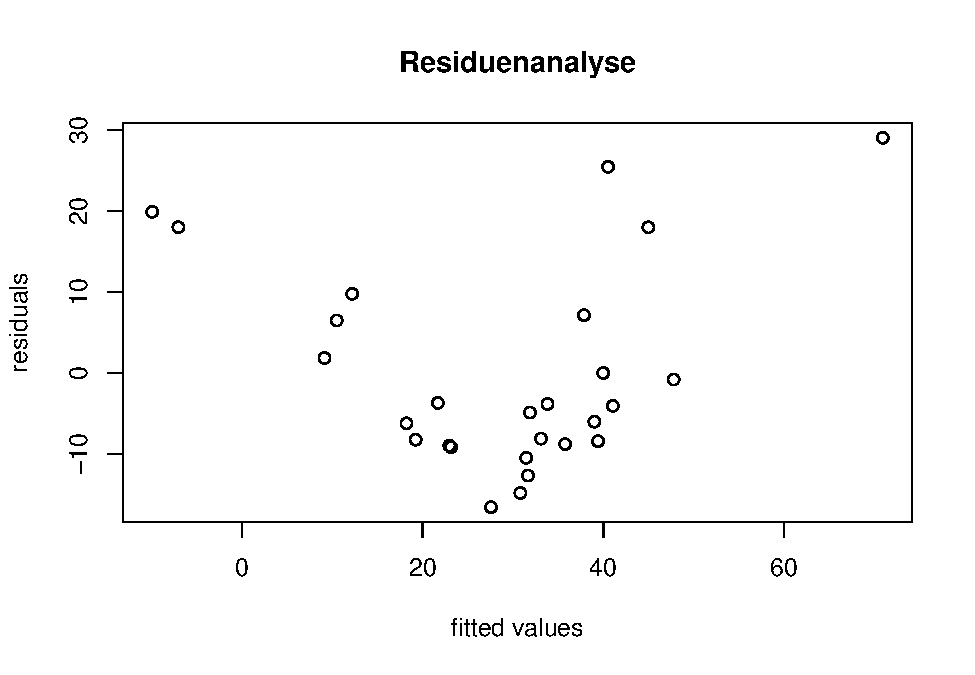
\includegraphics{Test_files/figure-latex/unnamed-chunk-20-1.pdf}
Die Residuen sind nicht unbedingt zufällig verteilt, man erkennt eine u-förmige Struktur. Das kann daran liegen, dass der
zufällige Fehler nicht unabhängig normalverteilt ist.

\hypertarget{lineares-log-modell}{%
\subsection{Lineares Log Modell}\label{lineares-log-modell}}

\begin{Shaded}
\begin{Highlighting}[]
\NormalTok{model3 <-}\StringTok{ }\KeywordTok{lm}\NormalTok{(}\KeywordTok{log}\NormalTok{(price) }\OperatorTok{~}\StringTok{ }\NormalTok{temp }\OperatorTok{+}\StringTok{ }\NormalTok{h.rain }\OperatorTok{+}\StringTok{ }\NormalTok{w.rain }\OperatorTok{+}\StringTok{ }\NormalTok{year, }\DataTypeTok{data =}\NormalTok{ data)}
\KeywordTok{summary}\NormalTok{(model3)}
\end{Highlighting}
\end{Shaded}

\begin{verbatim}
## 
## Call:
## lm(formula = log(price) ~ temp + h.rain + w.rain + year, data = data)
## 
## Residuals:
##     Min      1Q  Median      3Q     Max 
## -0.4450 -0.2362  0.0181  0.1888  0.5100 
## 
## Coefficients:
##               Estimate Std. Error t value Pr(>|t|)    
## (Intercept) 40.6777920 14.3374580   2.837  0.00959 ** 
## temp         0.6187109  0.0943199   6.560 1.35e-06 ***
## h.rain      -0.0037482  0.0007915  -4.736  0.00010 ***
## w.rain       0.0011972  0.0004740   2.526  0.01924 *  
## year        -0.0243519  0.0069947  -3.481  0.00212 ** 
## ---
## Signif. codes:  0 '***' 0.001 '**' 0.01 '*' 0.05 '.' 0.1 ' ' 1
## 
## Residual standard error: 0.2805 on 22 degrees of freedom
## Multiple R-squared:  0.8308, Adjusted R-squared:  0.8001 
## F-statistic: 27.01 on 4 and 22 DF,  p-value: 3.294e-08
\end{verbatim}

In der Summary steht nun auch der zufällige Fehler für die logarithmierten Daten. Um einen Vergleichbaren Wert zu erhalten,
müssen wir den geschätzten zufälligen Fehler für die normalen Daten berechnen:

\begin{Shaded}
\begin{Highlighting}[]
\NormalTok{true.fitted.values =}\StringTok{ }\KeywordTok{exp}\NormalTok{(model3}\OperatorTok{$}\NormalTok{fitted.values)}
\NormalTok{model3.sigma.hat.sq =}\StringTok{ }\KeywordTok{sum}\NormalTok{((data}\OperatorTok{$}\NormalTok{price }\OperatorTok{-}\StringTok{ }\NormalTok{true.fitted.values)}\OperatorTok{^}\DecValTok{2}\NormalTok{)}\OperatorTok{/}\NormalTok{(}\KeywordTok{length}\NormalTok{(data}\OperatorTok{$}\NormalTok{price)}\OperatorTok{-}\DecValTok{4}\NormalTok{)}
\KeywordTok{print}\NormalTok{(}\KeywordTok{paste}\NormalTok{(}\StringTok{"sigma.hat= "}\NormalTok{, }\KeywordTok{sqrt}\NormalTok{(model3.sigma.hat.sq)))}
\end{Highlighting}
\end{Shaded}

\begin{verbatim}
## [1] "sigma.hat=  8.41672958083313"
\end{verbatim}

\begin{Shaded}
\begin{Highlighting}[]
\NormalTok{model3.R2=}\DecValTok{1}\OperatorTok{-}\KeywordTok{sum}\NormalTok{((data}\OperatorTok{$}\NormalTok{price}\OperatorTok{-}\NormalTok{true.fitted.values)}\OperatorTok{^}\DecValTok{2}\NormalTok{)}\OperatorTok{/}\KeywordTok{sum}\NormalTok{((data}\OperatorTok{$}\NormalTok{price}\OperatorTok{-}\KeywordTok{mean}\NormalTok{(data}\OperatorTok{$}\NormalTok{price))}\OperatorTok{^}\DecValTok{2}\NormalTok{)}
\KeywordTok{print}\NormalTok{(}\KeywordTok{paste}\NormalTok{(}\StringTok{"R2= "}\NormalTok{, model3.R2))}
\end{Highlighting}
\end{Shaded}

\begin{verbatim}
## [1] "R2=  0.857300737700796"
\end{verbatim}

Die angepassten Werte sind immernoch besser als die der vorherigen Modelle.

\hypertarget{residuenanalyse-1}{%
\subsubsection{Residuenanalyse}\label{residuenanalyse-1}}

\begin{Shaded}
\begin{Highlighting}[]
\KeywordTok{plot}\NormalTok{(}\KeywordTok{exp}\NormalTok{(model3}\OperatorTok{$}\NormalTok{fitted.values), }\KeywordTok{exp}\NormalTok{(model3}\OperatorTok{$}\NormalTok{residuals), }\DataTypeTok{xlab =} \StringTok{"fitted values"}\NormalTok{, }\DataTypeTok{ylab =} \StringTok{"residuals"}\NormalTok{, }\DataTypeTok{main =} \StringTok{"Residuenanalyse"}\NormalTok{)}
\end{Highlighting}
\end{Shaded}

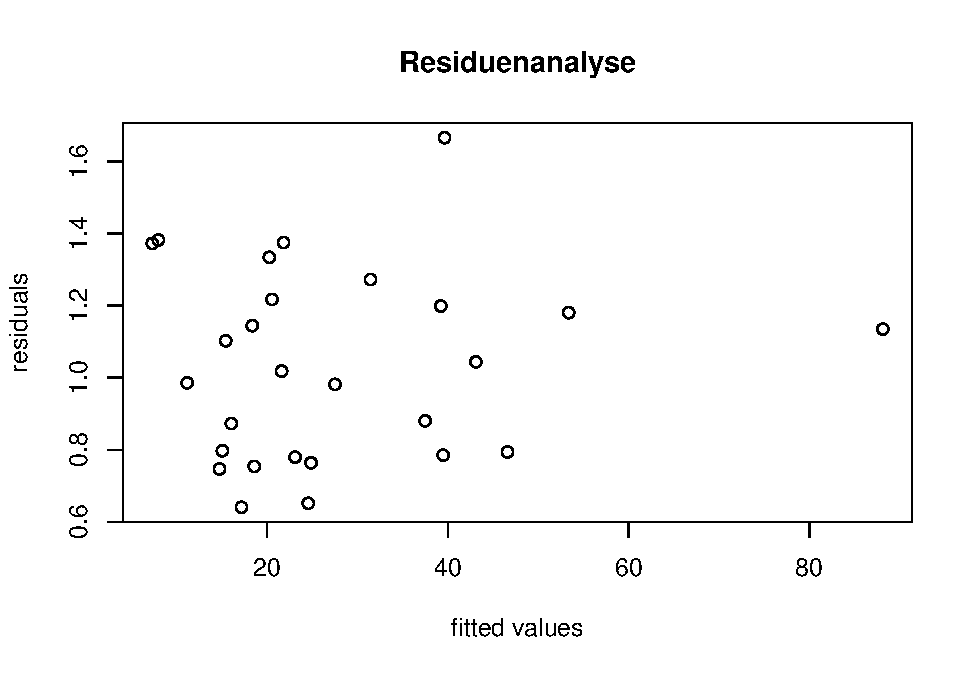
\includegraphics{Test_files/figure-latex/unnamed-chunk-23-1.pdf}
Sieht relativ unabhängig normalverteilt aus.\\
Vergleich mit Modell 2:
Modell 3 ist deutlich besser als Modell 2, da die Residuen von Modell 3 unabhängig normalverteilt wirken, und die von Modell 2 nicht.

\hypertarget{vergleich-der-3-modelle}{%
\subsection{Vergleich der 3 Modelle}\label{vergleich-der-3-modelle}}

\begin{Shaded}
\begin{Highlighting}[]
\NormalTok{Vergleichstabelle <-}\StringTok{ }\KeywordTok{data.frame}\NormalTok{(}
  \DataTypeTok{Model =} \KeywordTok{c}\NormalTok{(}\StringTok{"Model 1"}\NormalTok{, }\StringTok{"Model 2"}\NormalTok{, }\StringTok{"Model 3"}\NormalTok{),}
  \DataTypeTok{R2 =} \KeywordTok{c}\NormalTok{(}\KeywordTok{summary}\NormalTok{(model)}\OperatorTok{$}\NormalTok{r.squared, }\KeywordTok{summary}\NormalTok{(model2)}\OperatorTok{$}\NormalTok{r.squared, model3.R2),}
  \DataTypeTok{Adjusted.R2 =} \KeywordTok{c}\NormalTok{(}\KeywordTok{summary}\NormalTok{(model)}\OperatorTok{$}\NormalTok{adj.r.squared, }\KeywordTok{summary}\NormalTok{(model2)}\OperatorTok{$}\NormalTok{adj.r.squared,}
                  \DecValTok{1}\OperatorTok{-}\NormalTok{(}\DecValTok{1}\OperatorTok{-}\NormalTok{model3.R2)}\OperatorTok{*}\NormalTok{(}\KeywordTok{length}\NormalTok{(data}\OperatorTok{$}\NormalTok{price)}\OperatorTok{-}\DecValTok{1}\NormalTok{)}\OperatorTok{/}\NormalTok{(}\KeywordTok{length}\NormalTok{(data}\OperatorTok{$}\NormalTok{price)}\OperatorTok{-}\DecValTok{4}\NormalTok{)),}
  \DataTypeTok{Sigma =} \KeywordTok{c}\NormalTok{(}\KeywordTok{summary}\NormalTok{(model)}\OperatorTok{$}\NormalTok{sigma, }\KeywordTok{summary}\NormalTok{(model2)}\OperatorTok{$}\NormalTok{sigma, }\KeywordTok{sqrt}\NormalTok{(model3.sigma.hat.sq))}
\NormalTok{)}
\NormalTok{knitr}\OperatorTok{::}\KeywordTok{kable}\NormalTok{(Vergleichstabelle)}
\end{Highlighting}
\end{Shaded}

\begin{tabular}{l|r|r|r}
\hline
Model & R2 & Adjusted.R2 & Sigma\\
\hline
Model 1 & 0.6420890 & 0.5954049 & 13.32969\\
\hline
Model 2 & 0.7369089 & 0.6890742 & 11.68525\\
\hline
Model 3 & 0.8573007 & 0.8386878 & 8.41673\\
\hline
\end{tabular}

Das dritte Modell ist signifikant besser als die anderen beiden Modelle, das sieht man an der höheren Adjusted \(R^2\)
und dem kleineren geschätzten zufälligen Fehler.

\bibliography{StochastikAusarbeitung.bib}

\end{document}
